% Chapter discussion

\chapter{Introduction-5/10pagine} % Main chapter title

\label{Chapter2} % For referencing the chapter elsewhere, use \ref{Chapter4} 

%----------------------------------------------------------------------------------------

%1. Sequenziamento (mezza pagina)
%2. Modelli: genomica e pangenomica, facendo riferimento al problema reference based.
%3. come si codifica l'informazione: pangenoma (GFA) + bubble e vcf.
%4. HLA e polimorfico, complesso con modelli genomici 


%Grandezza genomi, genomi complessi, definizione pangenoma.

\section{Sequencing}
%mezza pagina

The process of sequencing determines the exact order of the monomers in a biomolecule, the nucleotides in the case of DNA sequencing. Sequence analyses has many applications, e.g. identify mutations or establish phylogenetic relationships among species.



Sanger's method marked the beginning of genomics research and has been successfully until a decade ago when next generation sequencing (NGS) was introduced to overcome the main limit of the Sanger sequencing, i.e. the sequencing volume. \\
NGS is an example  high-throughput sequencing. Unlike the traditional Sanger method, the NGS allows today to analyze many sequences in parallel, reducing analysis times and costs: the sequencing of the first human genome, based on the Sanger method, required an investment of almost 100 million dollars, while today the sequence of a human genome can be obtained for as little as $1,500$ dollars.
But NGS has some limitations: it requires the initial amplification of DNA sequences (which could introduce random errors in the sequence) and leads to the loss of "accessory" information, such as the constellation of epigenetic modifications that are important for understanding the function of a fragment of genome.\\

To overcome these limitations, research is now pointing towards third generation methods, such as nanopore sequencing. This technology derives from an observation that emerged as early as the 1980s: when a single-stranded DNA passes through a very narrow channel (nanopore) it generates a flow of ions with a characteristic pattern, which depends uniquely on its sequence. This technology would allow sequencing millions of nucleotides without resorting to the amplification of DNA fragments\\

AMPLIARE E METTERE REFERENZE 

\url{https://ib.bioninja.com.au/standard-level/topic-3-genetics/32-chromosomes/genome-size.html}
aggiungere questo concetto, complessità degli organismi in giga, trovare articolo.

\section{Genome \textit{versus} pangenome}


Genomics studies are based on two models: standard and alternative models. 

Standard approaches analysis relate sequences to a single linear reference genome. This is efficient but has a fundamental problems, i.e. differences from this reference are hard to observe and describe. Variation and sequence are separated. 

Alternative model i.e Pangenomic methods allow us to relate all genomes directly to each other. Sequence and variation are combined. This practice is still new, and research into ways to design, implement, and apply this model is ongoing. \\

In reference-based genomic analyses (\ref{fig:genomevspangenome.png} a), all genomes (A–D) are compared with each other via their relationship to the reference genome (R).
In a pangenomic analyses(\textbf{ii)},  all genomes are compared to each other, from which a particular reference is chosen arbitrarily. 
When extending the analysis with a new genome, (\textbf{iii}) one adds it to the genomic model by comparing it with the reference genome.
Instead in a pangenomic analyses,(\textbf{iv}), adding a new genome compares it directly with all other genomes in the model.\\
 
Regions of some genomes (\ref{fig:genomevspangenome.png} b) are unalignable against the reference and cannot be represented in a list of variants. A graphical model of the genomes allows a direct all-to-all comparison (\textbf{ii}), capturing all of their sequence relationships.

A collection of sequences representing a pangenome (\ref{fig:genomevspangenome.png} c). Multiple sequence alignment of the sequences captures their mutual relationships (\textbf{ii}).

(\ref{fig:genomevspangenome.png} d) In a de Bruijn graph, sequences are represented without bias, but variants may
correspond to larger graph structures. (\textbf{ii}) An acyclic sequence graph is equivalent to the multiple sequence alignment. (\textbf{iii}) A generic sequence graph can compactly represent a structural variant (shown in orange), using edges between the forward and reverse strands of
the graph to indicate the presence of an inversion.


\begin{figure}[H]
\centering
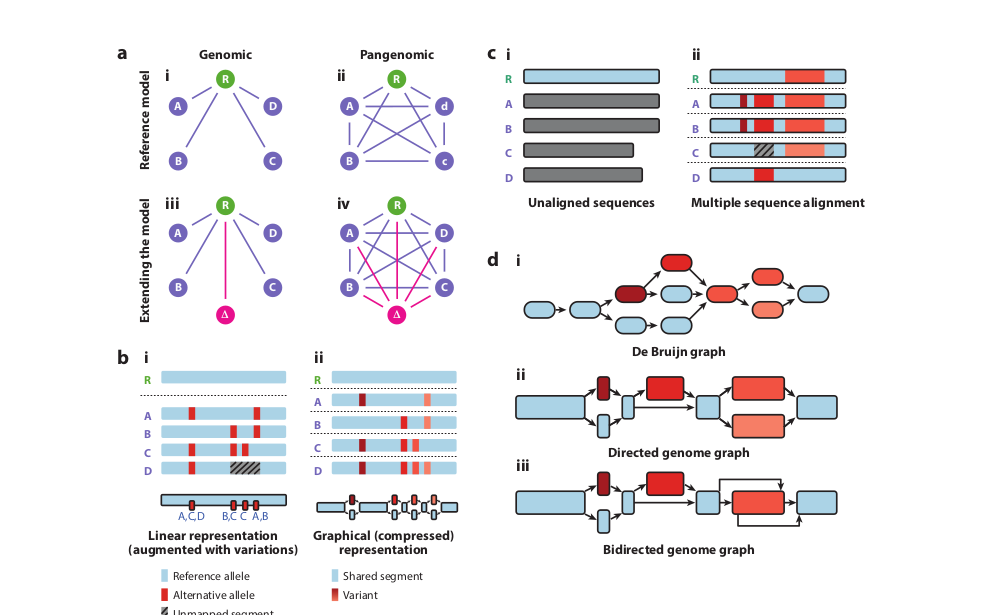
\includegraphics[width=1.00\textwidth]{fig/pangenome_genome.png}
\decoRule
\caption{Genomics versus pangenome (\textbf{A}), Linear representation with variants and Graphical representation compressed (\textbf{B})  Unaligned sequences and multiple sequence alignment (\textbf{C}), three types of graphs(\textbf{D}) CITARE FONTE }
\label{fig:genomevspangenome.png}
\end{figure}

\section{Bubbles}

Variants are coding in the graph as bubbles. 

\begin{figure}[H]
\centering
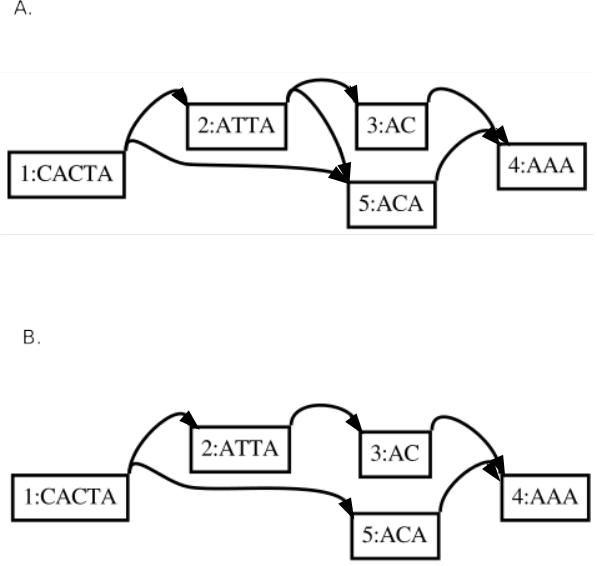
\includegraphics[width=0.50\textwidth]{fig/sup_bub.png}
\decoRule
\caption{Superbubble(\textbf{A}), Bubble (\textbf{B})}
\label{fig:sup_bub.png}
\end{figure}


The superbubble is a more complex subgraph type in which a set of (not necessarily disjoint) paths start and end at common source and sink nodes.\cite{paten2018superbubbles}.
Refering the definition from \cite{onodera2013detecting}, any pair of distinct vertices equation in a digraph (Fig: \ref{fig:sup_bub.png}A):

\begin{enumerate}
\item reachability: y is reachable from x.

\item matching: The set of vertices, X, reachable from x without passing through y is equal to the set of vertices from which y is reachable without passing through x (passing through here means to enter and then exit a vertex on the path).

\item acyclicity: The subgraph induced by X is acyclic.

\item minimality: No vertex in X other than y forms a pair with x that satisfies the criteria previously defined, and similarly for y.


\end{enumerate}

I'm concentred for \textit{bubblepop} to a case specific of a superbubble i.e  bubbles (Fig: \ref{fig:sup_bub.png})

A bubble consists of multiple directed unipaths from a vertex\textbf{ v} to a vertex \textbf{u} and is commonly caused by a small number of errors in the centre of reads.\cite{brankovic2016linear}. The bubble may be generalized to the idea of a superbubble, which is a directed, acyclic component of a graph with a single head and tail node.\cite{onodera2013detecting}.

A homologous sequence corresponding to the common start
and end nodes in the bubble flanks two or more alternative alleles in the middle.\cite{garrison2019graphical}.Bubbles can nest and contain more complicated internal structures between the paths
through them. 

\section{Coding of genetic information}

The genomic information is coded with linear model i.e Variant Call Format(VCF) and with Graphical representation of a pangenome(GFA).

\subsection{Variant Call Format}
Variant Call Format (VCF) is a text file format and is a generic format for storing DNA polymorphism data such as SNPs, insertions, deletions and structural variants, together with rich annotations. (\cite{10.1093/bioinformatics/btr330}). 


\begin{figure}[H]
\centering
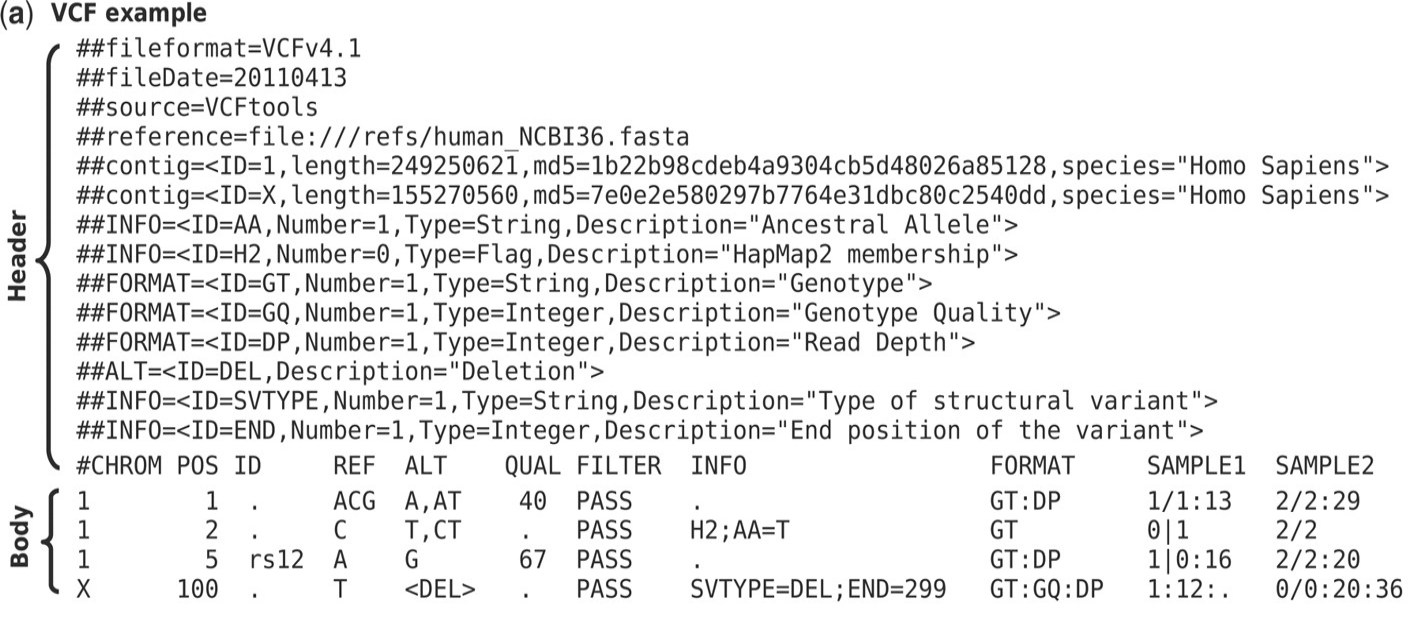
\includegraphics[width=1.00\textwidth]{fig/vcf.png}
\decoRule
\caption{AMPLIARE (\textbf{A}), Linear representation with variants (VCF)) Fig:\cite{10.1093/bioinformatics/btr330}}
\label{fig:vcf.png}
\end{figure}



VCF file (\ref{fig:vcf.png}) consists of:
\begin{itemize}

\item\textbf{Header section}

In the (Fig: \ref{fig:vcf.png}) adapted by (\cite{10.1093/bioinformatics/btr330}) the header contains an arbitrary number of information lines, each starting with characters \verb##, and a TAB delimited field definition line, starting with a single \verb#,
character. The meta-information header lines provide a standardized description of tags and annotations used in the data section. The use of meta-information allows the information stored within a VCF file to be tailored to the data set in question. It can be also used to provide information about the means of file creation, date of creation, version of the reference sequence, software used and any other information relevant to the history of the file. 

\item\textbf{Data column}

These corresponding to data columns representing the chromosome (CHROM), a 1-based position of the start of the variant (POS), unique identifiers of the variant (ID), the reference allele (REF), a comma separated list of alternate non-reference alleles (ALT), a phred-scaled quality score (QUAL), site filtering information (FILTER) and a semicolon separated list of additional, user extensible annotation (INFO). In addition, if samples are present in the file, the mandatory header columns are followed by a FORMAT column and an arbitrary number of sample IDs that define the samples included in the VCF file. The FORMAT column is used to define the information contained within each subsequent genotype column, which consists of a colon separated list of fields.

\end{itemize}


\subsection{Graphical Fragment Assembly}

\begin{figure}[H]
\centering
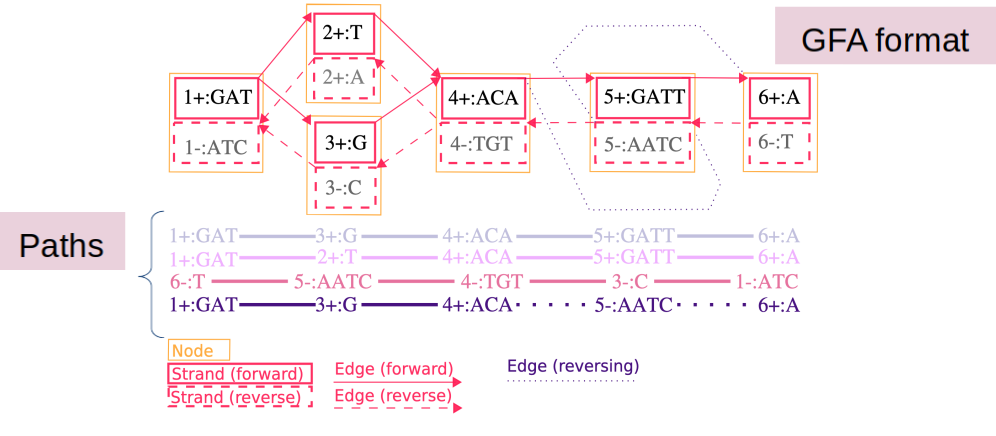
\includegraphics[width=1.00\textwidth]{fig/GFA.png}
\decoRule
\caption{Entities in the bidirected sequence graph (\textbf{A}) \cite{eizenga2020succinct}}
\label{fig:gfa.png}
\end{figure}

Pangenome data are represented by Graphical Fragment Assembly(GFA).

%per ENZA, spiegare handlegraph, nomi diversi ecc?

In the GFA, there are five elements important:
\begin{itemize}

\item\textbf{Nodes}

Nodes, (Fig: \ref{fig:gfa.png}) are represented by yellow rectangles. Each node is associated with a numeric ID and a sequence.  

\item\textbf{Strand Forward and reverse}

DNA strand has forward (+) and reverse (-) orientation. Handles show the node identifier, the direction (+ or -), and the sequence of the handle.  In (Fig: \ref{fig:gfa.png}) node contain a forward and reverse handle (red solid and dashed rectangles, respectively)

\item\textbf{Edges}				

Edges are shown as connections between nodes. In (Fig: \ref{fig:gfa.png}) are represented by the arrows between nodes. 

\item\textbf{Steps}

Steps describe paths visits to nodes strands.

\item\textbf{Paths} 

Paths indicate how the sequences walk in the gfa, all possible paths.


(Fig: \ref{fig:gfa.png}) the first two paths differ by a SNP, with one passing through 2+:T, and the other through 3+:G. The third path is the reverse complement of the first. The fourth is the same as the first, but contains an inversion, passing through 5-: AATC rather than 5+: GATT.
\end{itemize}



\section{HLA}

\begin{figure}[H]
\centering
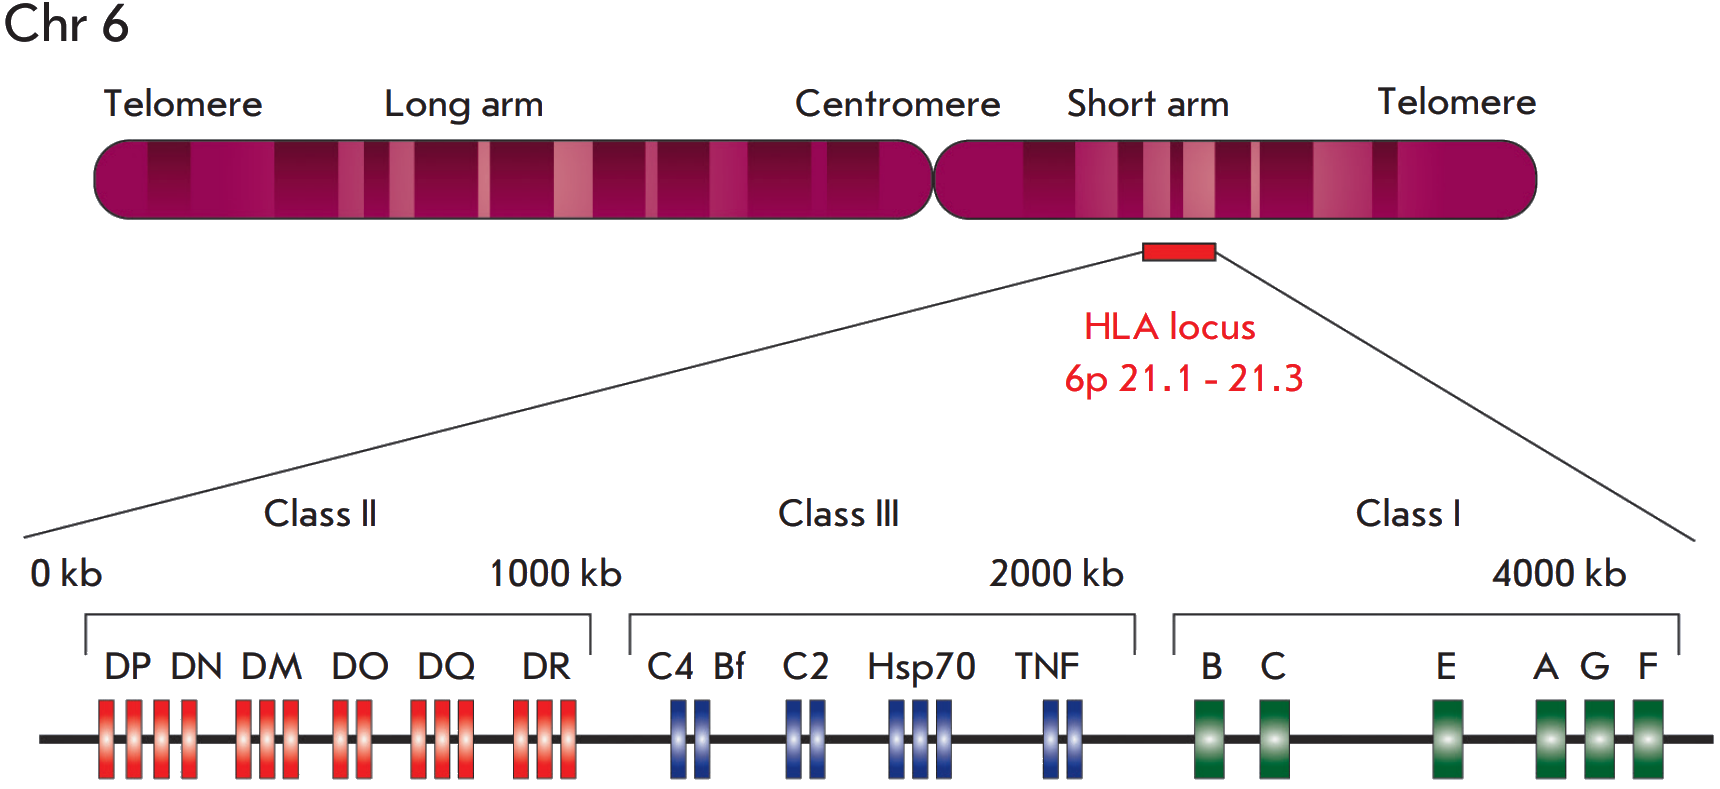
\includegraphics[width=0.80\textwidth]{fig/HLA_loci.png}
\decoRule
\caption{Schematic representation of the HLA locus on human chromosome 6. \cite{zakharova2019contribution})}
\label{fig:HLA.png}
\end{figure}

%mettere anche grafo corrispondente?

Genetic studies describes that an important roles in the developing of diseases is played by the major histocompatibility complex (MHC), or human leukocyte antigen (HLA). It contains several gene clusters that encode surface heterodimeric proteins, which are anchored to the plasma membrane and are responsible for antigen presentation to T cells, a stage that is followed by the development of an adaptive immune response. MHC proteins are subdivided into class I, class II, and class III (the complement system) \cite{campbell1993map}. \\



The HLA region (Fig.\ref{fig:HLA.png}) adapted by \cite{zakharova2019contribution} is located on the short arm of chromosome 6 from 6p21.1 to p21.3 and is shown with a red stripe. The length of class II (red), class III (blue), and class I (green) genes (from the centromeric to the telomeric end) is shown. The class II region includes genes for the {\ensuremath{\alpha}} and {\ensuremath{\beta}} chains of the MHC class II molecules HLA-DR, HLA-DP and HLA-DQ. In addition, the genes encoding the DMαand DM {\ensuremath{\beta}} chains, as well as the genes encoding the {\ensuremath{\alpha}} and {\ensuremath{\beta}} chains of the DO molecule (DO {\ensuremath{\alpha}} and DO{\ensuremath{\beta}}, respectively), are also located in the MHC class II region.\\




In the latest version \cite{eggertsson2017graphtyper} of the human reference genome (GRCh38), there are several alternate loci where the sequence variation is too complex to be represented with a single sequence. These loci are generally highly polymorphic, and many are known to co-segregate with disease and are therefore of great interest in population genetics. The most prominent example, the HLA region, is known to associate with a number of human diseases \cite{tiwari2012hla}. \\

Short-read sequencing is the standard in genome-wide sequence analysis. Most common approaches for discovering sequence variants involve aligning sequence reads to a reference genome \cite{li2009fast} and searching for variants as alternative sequences in read alignments. However, some reads cannot be aligned to a reference genome, particularly those originating from highly polymorphic regions and regions absent from the reference genome.